\documentclass[11pt,a4paper]{article}
\usepackage[utf8]{inputenc}
\usepackage[T1]{fontenc}
\usepackage[portuguese]{babel}
\usepackage{amsmath}
\usepackage{amsfonts}
\usepackage{amssymb}
\usepackage{geometry}
\usepackage{hyperref}
\geometry{a4paper, margin=2.5cm}
\usepackage{graphicx}
\graphicspath{{../experiments/plots/}}
\usepackage{float}

\title{Trabalho Prático 3 \\ Sistema de E-commerce com Consultas Multiatributo}
\author{Thales Alves Amaral \\ \small{Departamento de Ciência da Computação} \\ \small{Universidade Federal de Minas Gerais (UFMG)} \\ \small{Belo Horizonte - MG - Brasil}}
\date{}

\begin{document}
\maketitle

\section{Introdução}
Este documento descreve a implementação de um sistema de e-commerce para a plataforma MercadoDCC. O programa mantém usuários, produtos, compras válidas e reposições de estoque, processando os comandos de entrada em ordem e produzindo, para cada operação, a saída definida pelo enunciado.

Resumidamente, o problema consiste em armazenar diferentes tipos de entidades e responder consultas por múltiplos atributos. Em vez de permitir apenas buscas por identificadores únicos, o sistema deve recuperar, por exemplo, usuários de uma certa cidade, produtos de uma marca, compras feitas por determinado usuário ou reposições que envolveram um produto específico. Para isso, a ideia central da solução é manter índices invertidos, isto é, estruturas que associam cada valor de atributo ao conjunto de identificadores das entidades que possuem aquele valor.

A solução utiliza TADs para representar usuários, produtos, compras, reposições, listas de identificadores, índices invertidos, buffers de consulta e funções auxiliares. As entidades principais são armazenadas em vetores dinâmicos, aproveitando o fato de que seus identificadores são inteiros sequenciais atribuídos a partir de 0, possibilitando acesso em tempo constante. Para os atributos buscáveis, foram usadas tabelas hash que mapeiam valores de atributos para listas de identificadores. Como esses identificadores são inseridos na ordem de cadastro das entidades, as listas já ficam naturalmente em ordem crescente, o que facilita a combinação de filtros por interseção linear e a impressão dos resultados na ordem exigida. Compras e reposições também armazenam seus produtos em ordem crescente de identificador, mantendo a saída consistente sem exigir uma ordenação completa a cada consulta.

\section{Método}
O projeto foi implementado em C++11, usando programação orientada a objetos (POO) e tipos abstratos de dados (TADs). A estrutura é modular, separada em headers e arquivos de implementação. Cada módulo concentra uma responsabilidade simples dentro do sistema:

\begin{itemize}
    \item \textbf{Usuário, Produto, Compra e Reposição} - Representam as quatro entidades principais do enunciado. Todas possuem um identificador inteiro atribuído automaticamente pelo sistema, em ordem crescente a partir de 0.

    O TAD Usuário armazena nome, idade, cidade, estado e nacionalidade. Além desses dados fixos, ele mantém um histórico agregado dos produtos comprados por aquele usuário, guardando para cada produto a quantidade total comprada.

    O TAD Produto armazena nome, preço, quantidade em estoque, categoria, marca e condição. O preço é armazenado em centavos, como inteiro, para evitar problemas de arredondamento com números reais. O produto mantém um histórico agregado dos usuários que o compraram.

    Os TADs Compra e Reposição armazenam timestamp, valor informado na entrada, e os pares de produto e quantidade associados à operação. A Compra também guarda o identificador do usuário que a realizou. Como os itens são lidos em um buffer temporário no \texttt{main}, cada compra e reposição guarda sua própria cópia dos itens em um vetor dinâmico. Antes de armazenar esses itens, o sistema os ordena por identificador de produto usando Insertion Sort, escolhido pela fácil implementação e pelo baixo custo nesse cenário.

    \item \textbf{ListaIds} - Guarda a lista de identificadores associada a um valor de atributo dentro de um índice invertido. A estrutura foi implementada como vetor dinâmico, com redimensionamento quando a capacidade se esgota. Como os identificadores das entidades são atribuídos de forma crescente e inseridos nos índices no momento do registro, a lista já fica naturalmente ordenada. Essa escolha evita uma ordenação extra nas consultas e permite fazer interseções de filtros de forma linear.

    \item \textbf{IndiceInvertido} - TAD responsável por associar um valor de atributo a uma \texttt{ListaIds}. Internamente, ele usa uma tabela hash com sondagem linear. Cada posição da tabela guarda uma chave textual e a lista de identificadores que possuem aquele valor. Por exemplo, no índice de cidade dos usuários, a chave \texttt{BeloHorizonte} aponta para a lista dos usuários cadastrados nessa cidade.

    A tabela é redimensionada sempre que começa a ficar muito cheia, mantendo as buscas mais eficientes, pois a implementação mantém no máximo 50\% da tabela preenchida. Quando há colisão, a busca continua nas posições seguintes até encontrar a chave ou uma posição vazia. Essa escolha foi feita porque o objetivo principal das consultas é localizar rapidamente o conjunto de candidatos de cada filtro. Em média, a tabela hash permite encontrar esse conjunto em tempo constante.

    \item \textbf{Indices} - Agrupa, em structs simples, os índices invertidos usados por cada tipo de entidade. Cada agrupamento armazena os índices dos atributos buscáveis daquela entidade.

    \item \textbf{BuffersConsulta} - Armazena vetores temporários reutilizados durante consultas e durante a leitura dos itens de compras e reposições. Os buffers principais guardam os resultados parciais de filtros, o resultado final da consulta, um vetor auxiliar para interseção e um vetor de itens temporários. Essa estrutura evita alocações repetidas nas consultas, o que diminui o custo de operação do sistema.

    \item \textbf{Sistema} - Módulo central da implementação. Ele mantém os vetores dinâmicos de usuários, produtos, compras e reposições, além dos grupos de índices invertidos. Também concentra as operações de cadastro, registro de compra, registro de reposição e consulta.

    Nos cadastros de usuários e produtos, o sistema cria a entidade no próximo identificador disponível e atualiza os índices dos atributos buscáveis. Nas reposições, ele ordena os itens por produto, incrementa o estoque, armazena a entidade Reposição e atualiza os índices de timestamp e produto. Nas compras, primeiro verifica se todos os produtos possuem estoque suficiente. Se a compra for inválida, nada é alterado e a saída é apenas \texttt{C INV}. Se for válida, o sistema decrementa o estoque, atualiza os históricos agregados de usuários e produtos, armazena a Compra e atualiza os índices de timestamp, usuário e produto.

    As consultas seguem a mesma ideia geral. Para cada filtro, o sistema obtém a lista de identificadores correspondente. Quando o filtro é por id, não é necessário usar hash, pois o próprio identificador já é a posição da entidade no vetor principal, ou seja, acesso simples em tempo constante. Quando há mais de um filtro, os resultados são combinados por interseção. Como as listas estão ordenadas, o sistema percorre as duas listas ao mesmo tempo e só mantém os identificadores que aparecem em ambas.

    \item \textbf{Auxiliares} - Concentra pequenas funções de conversão e impressão. A função \texttt{precoParaCentavos} converte o preço textual da entrada para inteiro em centavos. A função \texttt{imprimirPreco} faz o caminho inverso na saída, sempre com duas casas decimais. Também há uma função para transformar inteiros em strings, usada para atributos numéricos, como idade e timestamp, nos índices invertidos.

    \item \textbf{Main} - Faz a leitura da entrada, o processamento sequencial dos comandos e a impressão das saídas.
\end{itemize}

\section{Análise de Complexidade}

\subsection{Variáveis utilizadas}

As variáveis utilizadas na análise são:

\begin{itemize}
    \item \(u\): número de usuários cadastrados;
    \item \(p\): número de produtos cadastrados;
    \item \(c\): número de compras válidas armazenadas;
    \item \(r\): número de reposições armazenadas;
    \item \(s\): número de itens em uma compra ou reposição;
    \item \(f\): número de filtros de uma consulta;
    \item \(k_i\): tamanho da lista de identificadores retornada pelo \(i\)-ésimo filtro;
    \item \(T_C\): número total de itens armazenados nas compras válidas;
    \item \(T_R\): número total de itens armazenados nas reposições.
\end{itemize}

As operações sobre tabelas hash são analisadas no caso médio, considerando que a tabela é redimensionada quando começa a ficar cheia. Assim, buscas e inserções nos índices invertidos têm custo médio constante, desconsiderando o tamanho das strings usadas como chave.

\subsection{Complexidade de espaço}

As entidades principais são armazenadas em vetores dinâmicos, ocupando espaço \(\mathcal{O}(u + p + c + r)\). Além disso, compras e reposições guardam seus respectivos itens, ocupando \(\mathcal{O}(T_C + T_R)\).

Os índices invertidos armazenam listas de identificadores para os valores dos atributos buscáveis. Como cada entidade é inserida em uma quantidade fixa de índices, e compras e reposições também são indexadas pelos produtos envolvidos, o espaço total dos índices é proporcional ao número de identificadores armazenados nessas listas. Assim, esse espaço é \(\mathcal{O}(u + p + c + r + T_C + T_R)\).

Os históricos agregados de usuários e produtos também dependem dos pares usuário-produto que aparecem nas compras válidas. No pior caso, esse espaço é \(\mathcal{O}(T_C)\), pois cada item comprado pode contribuir para os históricos. O fato de a informação ser mantida tanto pelo lado do usuário quanto pelo lado do produto altera apenas o fator constante.

Os buffers auxiliares usados nas consultas têm tamanho linear no maior conjunto consultado e não alteram a ordem assintótica total.

Portanto, somando os vetores principais, os itens armazenados, os índices invertidos, os históricos agregados e os buffers auxiliares, o espaço total utilizado pelo sistema é:

\[
\mathcal{O}(u + p + c + r + T_C + T_R)
\]

\subsection{Complexidade de tempo}

O cadastro de usuários e produtos insere uma entidade no vetor principal e atualiza uma quantidade fixa de índices invertidos. Como a inserção em vetor dinâmico tem custo amortizado constante, pois os redimensionamentos acontecem apenas ocasionalmente, e as operações na hash têm custo médio constante, os cadastros possuem custo médio:

\[
\mathcal{O}(1)
\]

O registro de uma reposição com \(s\) itens ordena os produtos por identificador usando Insertion Sort, com custo \(\mathcal{O}(s^2)\). Depois, percorre os itens para atualizar o estoque e os índices. Assim, o custo total é:

\[
\mathcal{O}(s^2)
\]

O registro de uma compra também ordena os \(s\) itens, valida o estoque e, caso a compra seja válida, atualiza estoque, índices e históricos agregados. A ordenação custa \(\mathcal{O}(s^2)\), e as atualizações percorrem os itens da compra. A atualização dos históricos pode exigir busca linear nas listas agregadas do usuário e dos produtos. Portanto, no pior caso, a compra pode custar:

\[
\mathcal{O}(s^2 + s(u+p))
\]

Na prática, como cada compra ou reposição costuma possuir poucos itens, os custos dessas operações tendem a ser menores do que os piores casos assintóticos indicados. Além disso, o Insertion Sort tem pior caso \(\mathcal{O}(s^2)\), mas se comporta próximo de \(\mathcal{O}(s)\) quando os itens já chegam ordenados ou quase ordenados.

As consultas LU, LP, LC e LR funcionam obtendo a lista de identificadores de cada filtro e combinando essas listas por interseção. A busca de cada filtro no índice invertido tem custo médio constante, e a interseção entre listas ordenadas é linear no tamanho das listas envolvidas. Assim, para uma consulta com \(f\) filtros, o custo é proporcional ao tamanho das listas retornadas:

\[
\mathcal{O}\left(\sum_{i=1}^{f} k_i\right)
\]

No pior caso, se os filtros forem pouco seletivos, essas listas podem conter quase todas as entidades consultadas. Assim, consultas sobre usuários podem chegar a \(\mathcal{O}(f \cdot u)\), sobre produtos a \(\mathcal{O}(f \cdot p)\), sobre compras a \(\mathcal{O}(f \cdot c)\) e sobre reposições a \(\mathcal{O}(f \cdot r)\).

Além disso, toda consulta possui o custo de impressão dos resultados, que é proporcional ao volume de dados impresso. Como os identificadores, históricos e itens são mantidos ordenados, não é necessário ordenar novamente antes da impressão.

\section{Estratégias de Robustez}

Como o enunciado trabalha com entradas válidas, a implementação não tenta corrigir formatos inesperados ou comandos inválidos. Mesmo assim, algumas decisões foram tomadas para evitar erros internos e manter o estado do sistema consistente ao longo da execução:

\begin{itemize}
    \item \textbf{Inicialização e destruição dos TADs:} Cada estrutura possui rotinas próprias de inicialização e liberação. Os contadores começam zerados, os ponteiros começam em estado conhecido e a memória alocada dinamicamente é liberada ao final da execução.

    \item \textbf{Redimensionamento dos vetores:} Os vetores dinâmicos aumentam de capacidade quando necessário, preservando os dados que já tinham sido inseridos. Isso evita acesso fora dos limites do array e permite que o programa aceite entradas maiores sem depender de um tamanho fixo escolhido antes.

    \item \textbf{Validação de compras:} Antes de efetivar uma compra, o sistema verifica se existe estoque suficiente para todos os itens. Caso a compra não seja válida, nenhuma alteração é feita no estoque, nos históricos ou nos índices invertidos, impedindo que uma operação parcial deixe o sistema inconsistente.

    \item \textbf{Consultas e impressão ordenada:} Os buffers usados nas consultas são reutilizados, mas sempre reiniciados antes de receber novos resultados. Além disso, as listas de identificadores são mantidas em ordem crescente, o que evita ordenações extras antes da impressão e reduz o risco de produzir saídas fora do formato esperado pelo VPL.
\end{itemize}



\section{Análise Experimental}

O objetivo central da análise experimental foi avaliar o comportamento da estrutura escolhida para responder consultas multiatributo. Como o projeto utiliza índices invertidos, os experimentos compararam o custo de atualização, o custo de consulta, o uso aproximado de memória e a localidade de referência de diferentes formas de armazenar e percorrer identificadores.

Para manter o programa submetido ao VPL separado do código de medição, os experimentos foram implementados em uma pasta separada do projeto. Foram utilizados scripts em Python para gerar gráficos (biblioteca \texttt{matplotlib}) e arquivos CSV com os dados, além de um programa de benchmark em C++, com a implementação das estruturas auxiliares usadas para comparação.

Foram comparadas três estratégias: busca sequencial em vetor, hash com vetor de identificadores e hash com lista encadeada de identificadores. A busca sequencial em vetor representa a solução mais simples, sem índices. A versão com hash e vetor corresponde à estrutura usada no projeto final. Já a versão com hash e lista encadeada foi incluída para avaliar o impacto da localidade de referência, comparando uma estrutura contígua em memória com uma estrutura baseada em ponteiros.

As entradas sintéticas variaram o número de registros gerados, o perfil de carga e a quantidade de filtros usados nas consultas, como recomendado pelo enunciado. Foram considerados três perfis principais: predominância de cadastros, predominância de compras e reposições, e predominância de consultas. Cada configuração foi executada cinco vezes, e o valor reportado corresponde à mediana das execuções, reduzindo o impacto de variações externas do sistema operacional.

Além dos tempos de execução e da estimativa de memória, foi feita uma análise de localidade de referência. Primeiro, comparou-se o tempo para percorrer identificadores armazenados em vetor e em lista encadeada. Em seguida, foi usado o Valgrind com a ferramenta Lackey, sugerida por um monitor da disciplina no fórum, para coletar uma amostra dos acessos à memória e visualizar as páginas acessadas ao longo da execução. Essa análise não substitui as medições de tempo, mas ajuda a explicar o desempenho prático observado entre vetor e lista encadeada. As próximas seções explicam os resultados mostrados em cada um dos 6 gráficos gerados.

\subsection{Perfis de carga}

A Figura~\ref{fig:tempo-perfil} compara as três estratégias nos perfis de carga usados no experimento. O eixo vertical está em escala logarítmica para facilitar a visualização, já que as diferenças entre as estratégias foram muito grandes em alguns cenários.

\begin{figure}[H]
\centering
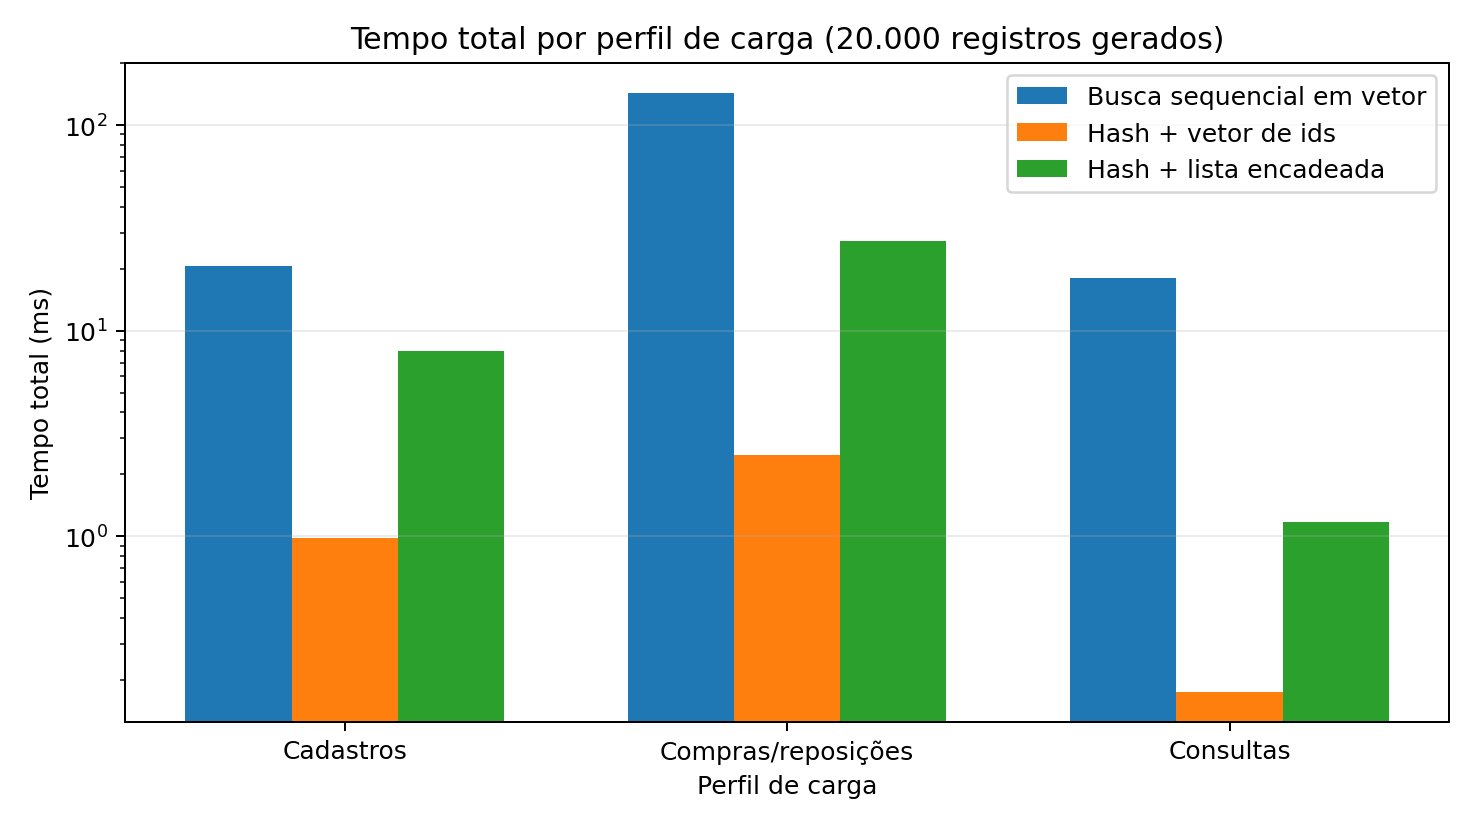
\includegraphics[width=0.7\linewidth]{01_tempo_por_perfil.png}
\caption{Tempo total por perfil de carga.}
\label{fig:tempo-perfil}
\end{figure}

No perfil com predominância de cadastros, a estratégia com hash e vetor de identificadores foi a mais rápida, levando cerca de 1{,}0 ms para 20 mil registros gerados. A busca sequencial em vetor levou aproximadamente 20{,}6 ms. Embora esse perfil tenha mais cadastros, ainda existem consultas na carga, e nelas a busca sequencial precisa percorrer muitos registros para testar os filtros, enquanto o uso de hash permite localizar diretamente os conjuntos de candidatos.

No perfil com predominância de compras e reposições, a diferença também foi clara. A estrutura com hash e vetor ficou em torno de 2{,}5 ms, enquanto a busca sequencial em vetor chegou a aproximadamente 143{,}9 ms. A lista encadeada ficou em uma posição intermediária, com cerca de 27{,}4 ms. Isso indica que o custo de manter os índices é compensado pelo ganho obtido nas consultas feitas ao longo da carga.

O perfil com predominância de consultas foi o caso em que a escolha da estrutura ficou ainda mais evidente. A versão com hash e vetor levou cerca de 0{,}18 ms, contra 18{,}0 ms da busca sequencial em vetor. A lista encadeada também foi melhor que a busca sequencial por usar índice invertido, mas ficou mais lenta que o vetor. Isso sugere que, além de usar índices, também importa como as listas de identificadores são armazenadas: o vetor permite percorrer os identificadores de forma contígua, enquanto a lista encadeada depende de acessos por ponteiros. A análise de localidade de referência apresentada mais à frente ajuda a explicar esse comportamento.

Em suma, o primeiro experimento confirma a decisão principal da implementação. A busca sequencial em vetor é simples, mas seu custo cresce quando as consultas aparecem com frequência. O índice invertido reduz bastante esse custo, e a versão com vetor de identificadores foi a mais eficiente nos três perfis avaliados.

\subsection{Crescimento do número de registros}

A Figura~\ref{fig:consultas-escala} mostra o tempo médio das consultas quando o número de registros gerados aumenta. Nesse experimento, as consultas usam dois filtros, mantendo o mesmo padrão de carga para as três estratégias avaliadas.

\begin{figure}[H]
\centering
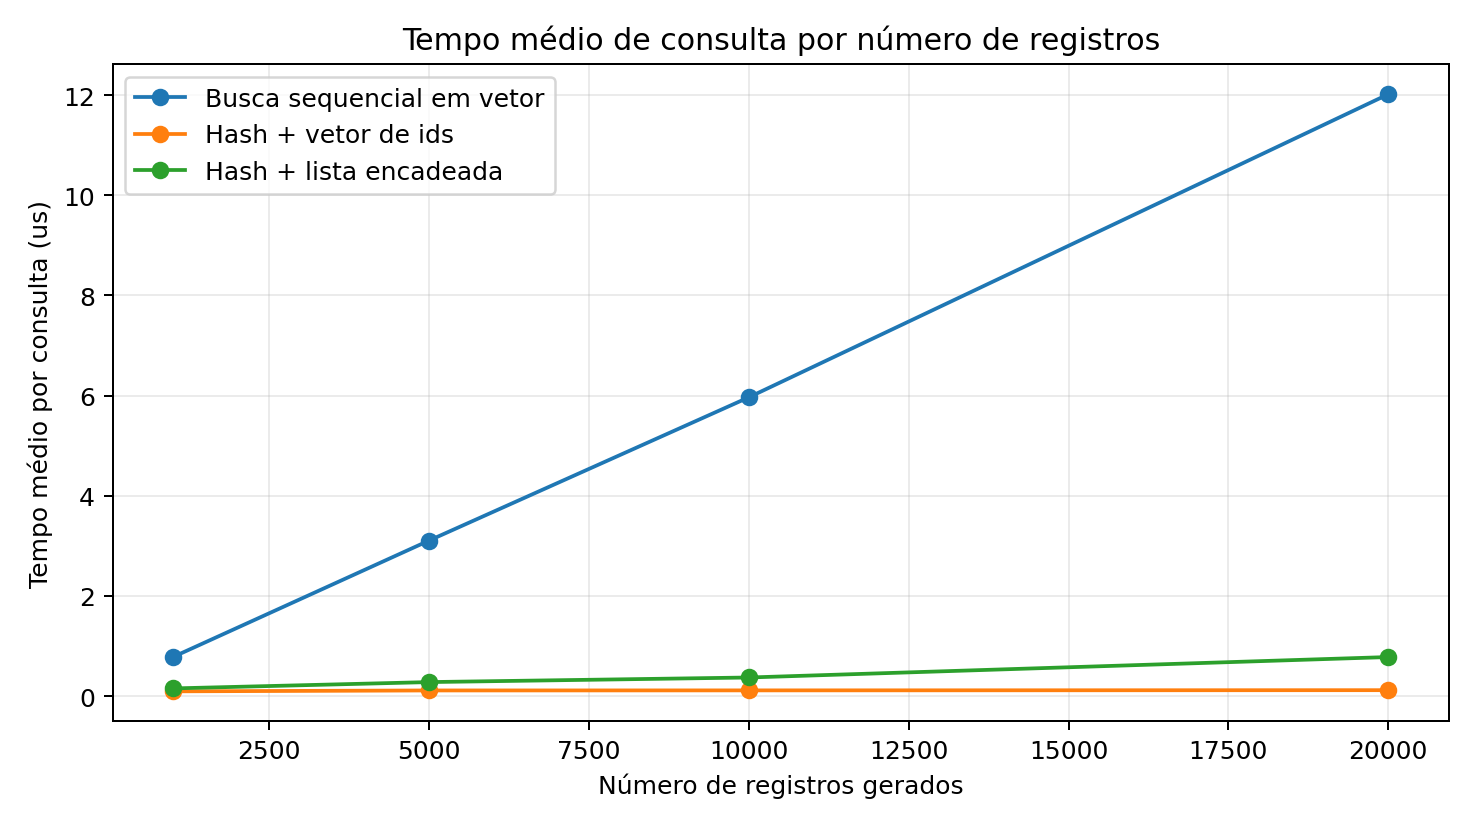
\includegraphics[width=0.7\linewidth]{02_consultas_por_escala.png}
\caption{Tempo médio de consulta por número de registros.}
\label{fig:consultas-escala}
\end{figure}

O comportamento da busca sequencial em vetor cresce quase linearmente com o número de registros. Com 1.000 registros, o tempo médio por consulta foi de aproximadamente 0{,}78 microssegundos. Com 20 mil registros, esse valor subiu para cerca de 12{,}02 microssegundos. Isso acontece porque, nessa estratégia, cada consulta precisa percorrer os registros e testar os filtros um por um.

As duas versões com índice invertido cresceram bem menos. A estratégia com hash e vetor ficou próxima de 0{,}1 microssegundos por consulta em todos os tamanhos testados. Isso acontece porque a consulta não percorre todos os registros: ela localiza diretamente as listas associadas aos filtros e trabalha apenas com os identificadores candidatos. A versão com lista encadeada também se beneficiou do índice invertido, mas foi mais lenta que o vetor por causa da pior localidade de referência, chegando a aproximadamente 0{,}78 microssegundos com 20 mil registros.


\subsection{Quantidade de filtros}

A Figura~\ref{fig:consultas-filtros} mostra o tempo médio das consultas quando a quantidade de filtros aumenta. Nesse experimento, o número de registros gerados foi mantido em 20 mil, variando apenas a quantidade de atributos usados em cada consulta.

\begin{figure}[H]
\centering
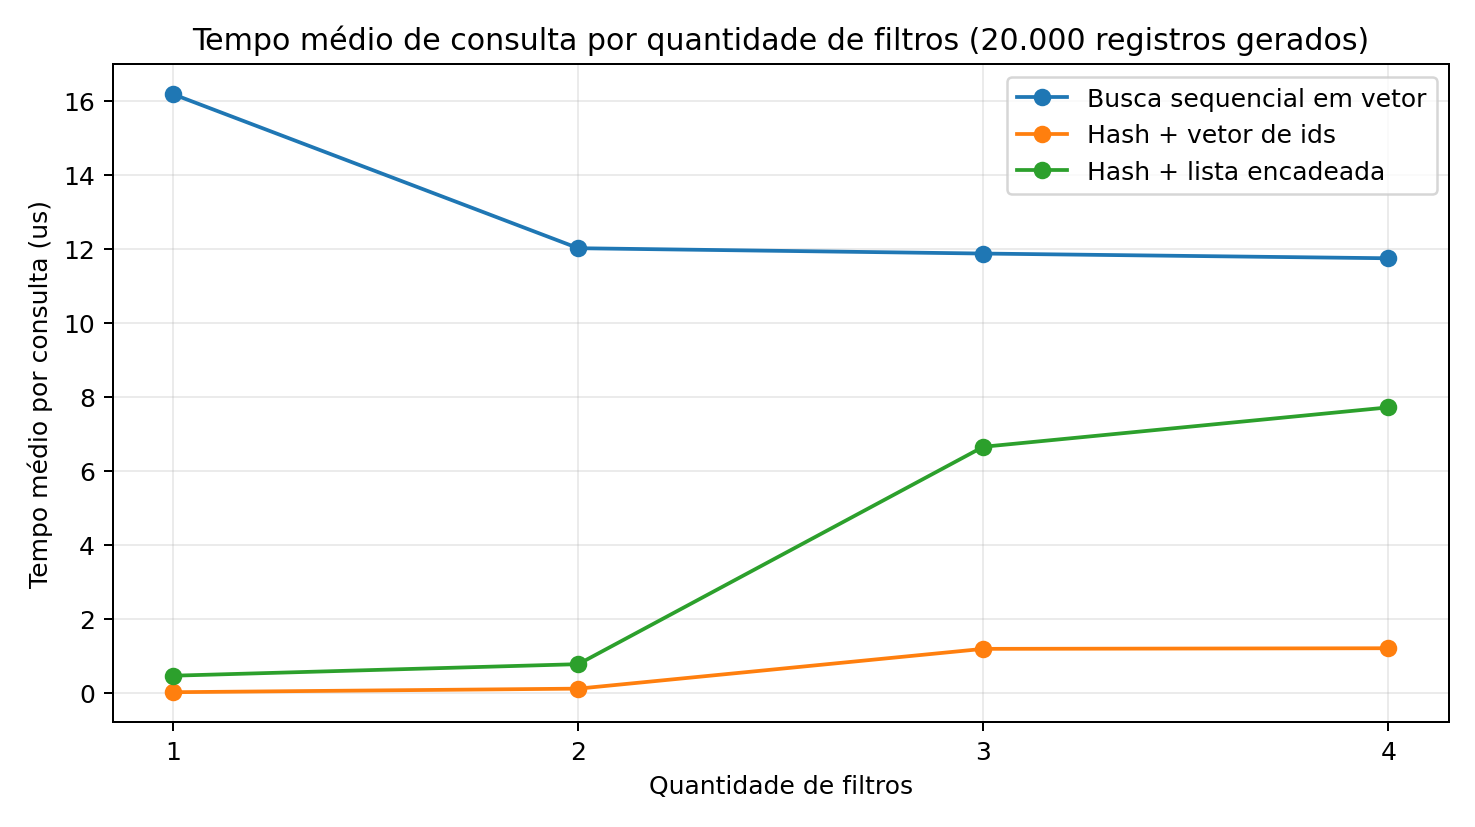
\includegraphics[width=0.7\linewidth]{03_consultas_por_filtros.png}
\caption{Tempo médio de consulta por quantidade de filtros.}
\label{fig:consultas-filtros}
\end{figure}

Na busca sequencial em vetor, o tempo ficou praticamente constante em relação à quantidade de filtros, sem apresentar uma tendência de crescimento. Os valores variaram de aproximadamente 16{,}17 microssegundos com um filtro para 11{,}74 microssegundos com quatro filtros, diferença que pode ser entendida como oscilação da medição. Isso acontece porque o custo principal dessa estratégia não está na quantidade de filtros, mas sim em percorrer todos os registros. Mesmo com mais filtros, o vetor ainda precisa ser examinado para descobrir quais registros satisfazem a consulta.

Nas estratégias com índice invertido, o aumento da quantidade de filtros teve impacto maior. A versão com hash e vetor passou de cerca de 0{,}02 microssegundos com um filtro para aproximadamente 1{,}21 microssegundos com quatro filtros. Já a versão com hash e lista encadeada passou de cerca de 0{,}47 para 7{,}72 microssegundos. Isso ocorre porque cada filtro adiciona uma nova lista de identificadores, e o sistema precisa combinar essas listas para formar a resposta final.

\subsection{Uso aproximado de memória}

A Figura~\ref{fig:memoria} mostra a estimativa de memória das três estratégias conforme o número de registros gerados aumenta. Essa medição não representa exatamente o consumo total do processo, mas sim uma estimativa das estruturas principais usadas em cada estratégia.

\begin{figure}[H]
\centering
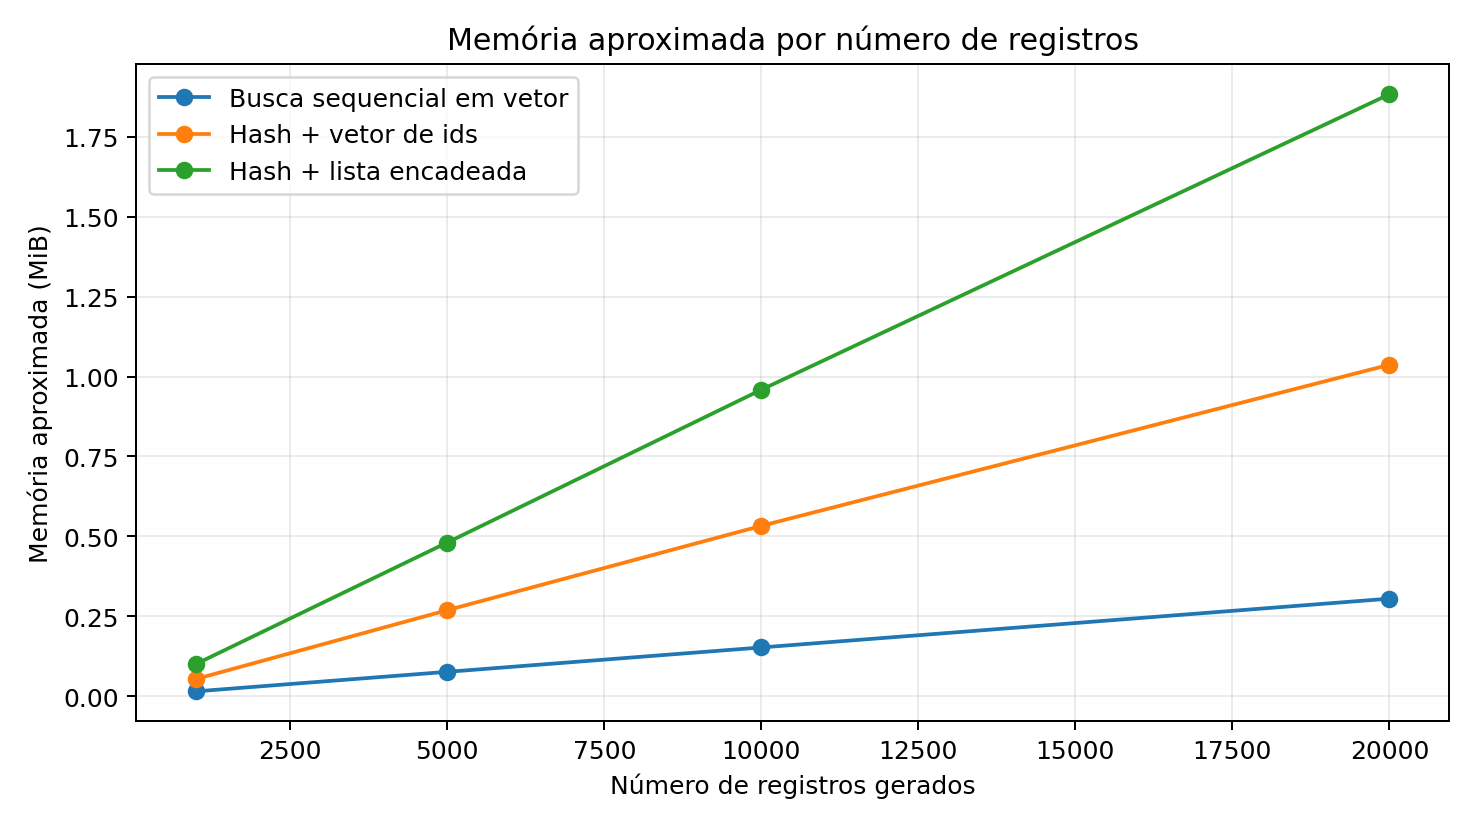
\includegraphics[width=0.7\linewidth]{04_memoria_aproximada.png}
\caption{Memória aproximada por número de registros.}
\label{fig:memoria}
\end{figure}

A busca sequencial em vetor foi a estratégia que utilizou menos memória, chegando a aproximadamente 0{,}31 MiB com 20 mil registros. Isso acontece porque ela armazena apenas os registros principais, sem manter índices auxiliares para acelerar as consultas.

As estratégias com hash usaram mais memória, como esperado. Com 20 mil registros, a versão com hash e vetor ficou em torno de 1{,}04 MiB, enquanto a versão com hash e lista encadeada chegou a aproximadamente 1{,}88 MiB. A diferença aparece porque, além da tabela hash, os índices precisam armazenar os identificadores associados a cada valor de atributo. No caso da lista encadeada, ainda existe o custo extra dos nós e ponteiros.

Em suma, o quarto experimento mostra o principal custo da escolha feita no projeto. O índice invertido melhora bastante o tempo das consultas, mas exige memória adicional. Entre as duas versões indexadas, o vetor de identificadores foi a alternativa mais interessante, pois manteve consultas mais rápidas e também consumiu menos memória que a lista encadeada.

\subsection{Localidade de referência}

A Figura~\ref{fig:localidade-tempo} compara o tempo para percorrer identificadores armazenados em vetor e em lista encadeada.

\begin{figure}[H]
\centering
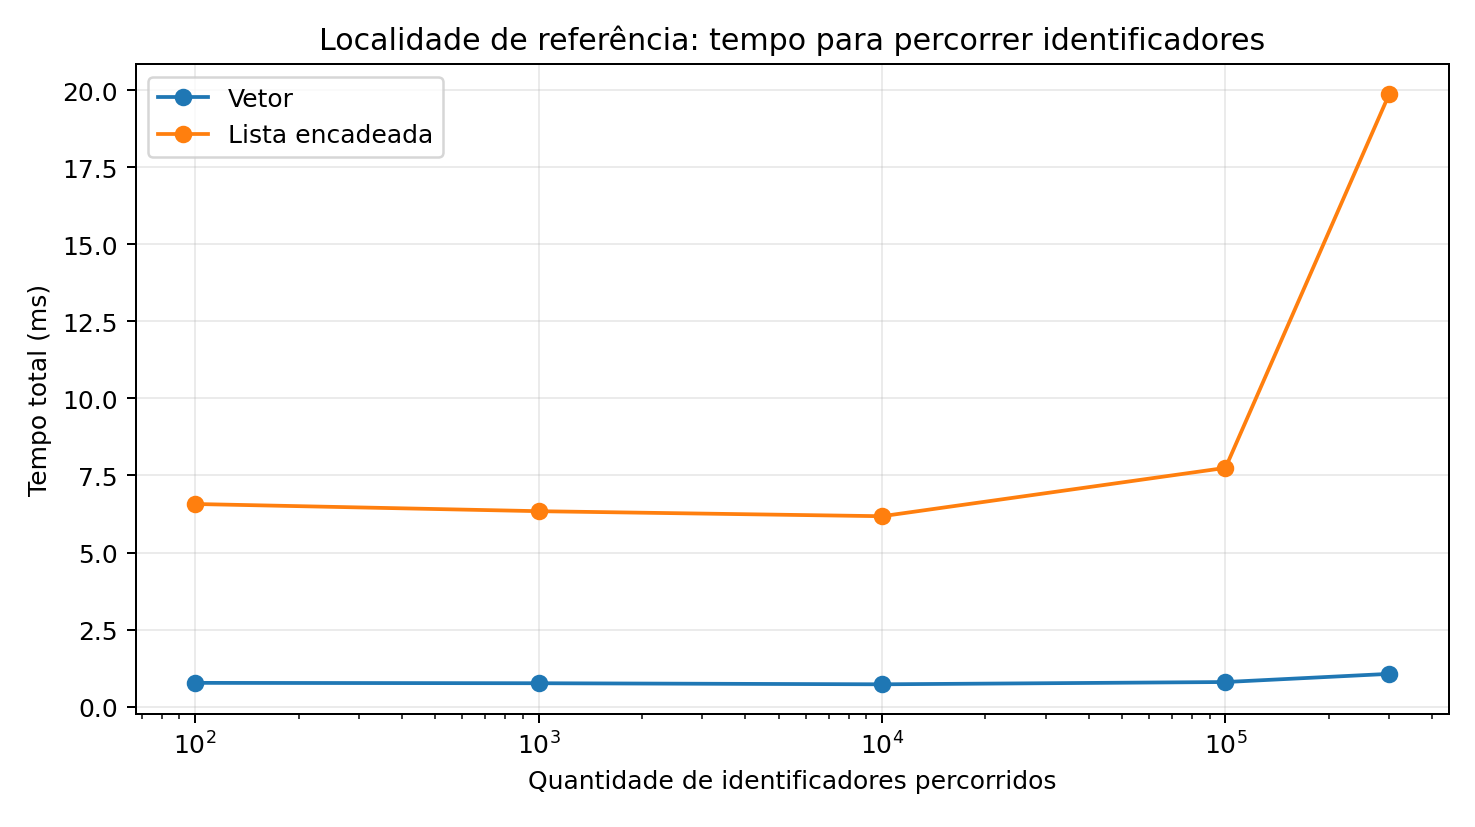
\includegraphics[width=0.7\linewidth]{05_localidade_tempo.png}
\caption{Tempo para percorrer identificadores.}
\label{fig:localidade-tempo}
\end{figure}

O vetor foi mais rápido em todos os tamanhos testados. No maior caso, o percurso em vetor levou cerca de 1{,}07 ms, contra aproximadamente 19{,}88 ms da lista encadeada. Embora as duas estruturas armazenem os mesmos valores, o vetor permite acessos contíguos em memória, enquanto a lista depende de ponteiros para chegar ao próximo nó.

\begin{figure}[H]
\centering
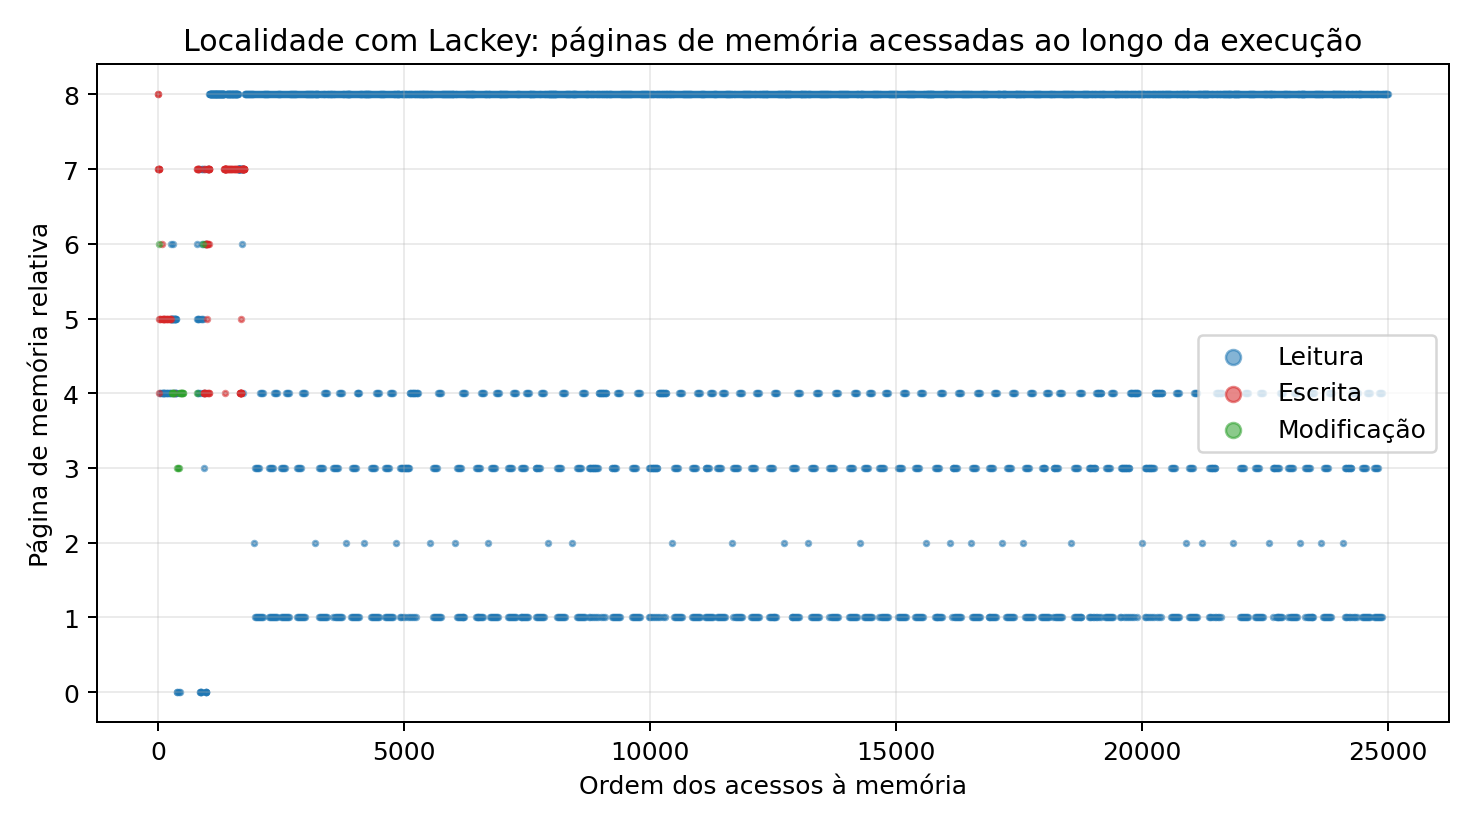
\includegraphics[width=0.7\linewidth]{06_localidade_trace.png}
\caption{Ordem de acesso e posição de memória.}
\label{fig:localidade-trace}
\end{figure}

A Figura~\ref{fig:localidade-trace} ajuda a visualizar esse comportamento. No vetor, os acessos aparecem em um padrão mais regular, indicando avanço por posições próximas de memória. Na lista encadeada, aparecem saltos entre regiões diferentes, o que reduz a localidade espacial. Resumindo, esses dois gráficos explicam por que, mesmo usando a mesma ideia de índice invertido, a versão com vetor de identificadores foi mais eficiente que a versão com lista encadeada e, portanto, foi escolhida como implementação do projeto final.

\section{Conclusões}

Este trabalho implementou um sistema de consultas multiatributo usando TADs próprios para representar usuários, produtos, compras, reposições, listas de identificadores e índices invertidos. A estrutura principal escolhida foi a tabela hash associada a vetores de identificadores, pois ela permite localizar rapidamente os candidatos de cada filtro e combinar os resultados sem percorrer todas as entidades armazenadas.

A principal troca dessa escolha é o uso adicional de memória. A busca sequencial em vetor é mais simples e ocupa menos espaço, mas se torna cara quando as consultas aparecem com frequência ou quando o número de registros cresce. Já o índice invertido exige manter estruturas auxiliares atualizadas nos cadastros, compras e reposições, mas reduz bastante o custo das consultas. Entre vetor e lista encadeada para guardar os identificadores, o vetor foi mais adequado por ter menor custo de memória e melhor localidade de referência.

Os experimentos reforçaram que a estratégia usada no projeto foi mais eficiente nos perfis avaliados, principalmente nos cenários com muitas consultas. A análise de localidade também ajudou a explicar o desempenho observado: percorrer dados contíguos em memória foi mais rápido do que seguir ponteiros em uma lista encadeada.

Em suma, a solução apresenta uma arquitetura simples, modular e resolve o problema proposto pelo enunciado. As principais dificuldades foram pensar e implementar o índice invertido usando hashing, garantindo que cada atributo consultável apontasse corretamente para os identificadores relacionados e a análise experimental, que exigiu a implementação de outras estratégias e a comparação entre elas. A partir disso, a parte mais importante foi equilibrar desempenho de consulta, custo de atualização, uso de memória e simplicidade da implementação.


\section{Bibliografia}
\begin{thebibliography}{9}
\bibitem{tp32026}
Anísio, Gisele, Wagner, Márcio (2026). \textit{Trabalho Prático 3: Sistema de E-commerce com Consultas Multiatributo}. Disponibilizado via Moodle. Departamento de Ciência da Computação. Universidade Federal de Minas Gerais. Belo Horizonte.
\bibitem{edslides2026}
Anísio, Gisele, Wagner, Márcio (2026). \textit{Slides da disciplina de Estrutura de Dados}. Disponibilizado via Moodle. Departamento de Ciência da Computação. Universidade Federal de Minas Gerais. Belo Horizonte.
\bibitem{abdulbari_channel}
BARI, Abdul. \textit{Abdul Bari - YouTube Channel}. Disponível em: <\url{https://www.youtube.com/@abdul_bari}>. Acesso em: 15 maio 2026.
\bibitem{geeksforgeeks_hash}
GEEKSFORGEEKS. \textit{Hash Table Data Structure}. GeeksforGeeks, 2025. 
Disponível em: https://www.geeksforgeeks.org/dsa/hash-table-data-structure/. 
Acesso em: 26 jun. 2026.
\end{thebibliography}
\end{document}